\documentclass[11pt,a4paper]{article}
\usepackage[utf8]{inputenc}
\usepackage[T1]{fontenc}
\usepackage[brazil]{babel}
\usepackage{lmodern}
\usepackage{amsmath,amssymb,bm}
\usepackage{graphicx,booktabs,float,geometry,url,array,xcolor,caption}
\usepackage[hidelinks]{hyperref}
\geometry{margin=2.2cm}
\captionsetup{font=small}
\emergencystretch=2em
\providecommand{\versao}{sem versão}
% gerado por gera_dados.py; nao edite
\newcommand{\fsDet}{1{,}5785}
\newcommand{\fsDetTres}{1{,}578}
\newcommand{\difDet}{3{,}5}
\newcommand{\difDetRel}{3{,}4}
\newcommand{\fsSemSuccao}{1{,}518}
\newcommand{\fsVert}{1{,}5782}
\newcommand{\fsFinal}{1{,}5764}
\newcommand{\fsTquatro}{1{,}5783}
\newcommand{\fsAevZero}{1{,}5728}
\newcommand{\fsXiZeroDois}{1{,}531}
\newcommand{\fsXiZeroTres}{1{,}525}
\newcommand{\nivelXX}{5{,}14}
\newcommand{\nivelLiuXX}{5{,}13}
\newcommand{\succXX}{13{,}2}
\newcommand{\succLiuXX}{14{,}7}
\newcommand{\difSatXX}{0{,}7}
\newcommand{\difMaxXX}{1{,}4}
\newcommand{\nivelYY}{4{,}56}
\newcommand{\nivelLiuYY}{4{,}56}
\newcommand{\succYY}{13{,}0}
\newcommand{\succLiuYY}{14{,}2}
\newcommand{\difSatYY}{0{,}0}
\newcommand{\difMaxYY}{1{,}4}
\newcommand{\betaDois}{4{,}82}
\newcommand{\pfFORMDois}{\ensuremath{7{,}1\times 10^{-7}}}
\newcommand{\alfaPhiDois}{0{,}85}
\newcommand{\alfaCDois}{0{,}15}
\newcommand{\pfLSDois}{\ensuremath{9{,}3\times 10^{-6}}}
\newcommand{\cvLSDois}{54}
\newcommand{\linhasDois}{600}
\newcommand{\anLSDois}{1\,447}
\newcommand{\anLinhaDois}{2{,}41}
\newcommand{\betaLSDois}{4{,}28}
\newcommand{\icLSloDois}{\ensuremath{3{,}5\times 10^{-6}}}
\newcommand{\icLShiDois}{\ensuremath{2{,}5\times 10^{-5}}}
\newcommand{\nMCDois}{2\,500}
\newcommand{\nfMCDois}{0}
\newcommand{\wilsonDois}{\ensuremath{1{,}5\times 10^{-3}}}
\newcommand{\muDois}{1{,}550}
\newcommand{\sdDois}{0{,}155}
\newcommand{\cvDois}{10{,}0}
\newcommand{\minMCDois}{1{,}122}
\newcommand{\assimDois}{0{,}32}
\newcommand{\betaLNDois}{4{,}35}
\newcommand{\pfLNDois}{\ensuremath{6{,}9\times 10^{-6}}}
\newcommand{\pfNDois}{\ensuremath{1{,}9\times 10^{-4}}}
\newcommand{\razaoLNLSDois}{0{,}74}
\newcommand{\betaLNredDois}{4{,}00}
\newcommand{\pfLNredDois}{\ensuremath{3{,}1\times 10^{-5}}}
\newcommand{\pfNredDois}{\ensuremath{4{,}4\times 10^{-4}}}
\newcommand{\redReqDois}{3{,}9}
\newcommand{\dbetaDois}{10{,}0}
\newcommand{\liuMuDois}{1{,}489}
\newcommand{\liuSdDois}{0{,}148}
\newcommand{\liuCvDois}{10{,}0}
\newcommand{\liuMinDois}{1{,}05}
\newcommand{\liuPfNDois}{\ensuremath{5{,}0\times 10^{-4}}}
\newcommand{\razaoTabQuatroDois}{4{,}4}
\newcommand{\razaoTabQuatroLNDois}{5{,}9}
\newcommand{\razaoTabQuatroRedDois}{1{,}3}
\newcommand{\pZeroTabDoisDois}{\ensuremath{4{,}4\times 10^{-5}}}
\newcommand{\pZeroTabQuatroDois}{0{,}90}
\newcommand{\nTabDoisDois}{10}
\newcommand{\razaoFORMDois}{13}
\newcommand{\nCquatroDois}{13}
\newcommand{\fracCquatroDois}{80}
\newcommand{\fracBaseDois}{93}
\newcommand{\razaoNLSDois}{21}
\newcommand{\razaoTabDoisRedDois}{127}
\newcommand{\fracMaiorDois}{51}
\newcommand{\fracDezDois}{78}
\newcommand{\cMinDois}{2{,}77}
\newcommand{\cMaxDois}{7{,}42}
\newcommand{\cMedDois}{5{,}00}
\newcommand{\cPcincoDois}{4{,}20}
\newcommand{\cPnoventaDois}{5{,}66}
\newcommand{\tempoDois}{132}
\newcommand{\nivXXmuDois}{5{,}10}
\newcommand{\nivXXsdDois}{0{,}00}
\newcommand{\nivXXloDois}{5{,}1}
\newcommand{\nivXXhiDois}{5{,}1}
\newcommand{\nivYYmuDois}{4{,}50}
\newcommand{\nivYYsdDois}{0{,}00}
\newcommand{\nivYYloDois}{4{,}5}
\newcommand{\nivYYhiDois}{4{,}5}
\newcommand{\betaTres}{4{,}77}
\newcommand{\pfFORMTres}{\ensuremath{9{,}3\times 10^{-7}}}
\newcommand{\alfaPhiTres}{0{,}85}
\newcommand{\alfaCTres}{0{,}15}
\newcommand{\pfLSTres}{\ensuremath{2{,}6\times 10^{-5}}}
\newcommand{\cvLSTres}{34}
\newcommand{\linhasTres}{600}
\newcommand{\anLSTres}{1\,433}
\newcommand{\anLinhaTres}{2{,}39}
\newcommand{\betaLSTres}{4{,}04}
\newcommand{\icLSloTres}{\ensuremath{1{,}4\times 10^{-5}}}
\newcommand{\icLShiTres}{\ensuremath{5{,}0\times 10^{-5}}}
\newcommand{\nMCTres}{10\,000}
\newcommand{\nfMCTres}{0}
\newcommand{\wilsonTres}{\ensuremath{3{,}8\times 10^{-4}}}
\newcommand{\muTres}{1{,}538}
\newcommand{\sdTres}{0{,}159}
\newcommand{\cvTres}{10{,}4}
\newcommand{\minMCTres}{1{,}036}
\newcommand{\assimTres}{0{,}33}
\newcommand{\betaLNTres}{4{,}11}
\newcommand{\pfLNTres}{\ensuremath{2{,}0\times 10^{-5}}}
\newcommand{\pfNTres}{\ensuremath{3{,}7\times 10^{-4}}}
\newcommand{\razaoLNLSTres}{0{,}74}
\newcommand{\betaLNredTres}{3{,}78}
\newcommand{\pfLNredTres}{\ensuremath{7{,}8\times 10^{-5}}}
\newcommand{\pfNredTres}{\ensuremath{8{,}0\times 10^{-4}}}
\newcommand{\redReqTres}{4{,}4}
\newcommand{\dbetaTres}{9{,}7}
\newcommand{\liuMuTres}{1{,}478}
\newcommand{\liuSdTres}{0{,}155}
\newcommand{\liuCvTres}{10{,}5}
\newcommand{\liuMinTres}{1{,}02}
\newcommand{\liuPfNTres}{\ensuremath{1{,}0\times 10^{-3}}}
\newcommand{\razaoTabQuatroTres}{4{,}5}
\newcommand{\razaoTabQuatroLNTres}{6{,}1}
\newcommand{\razaoTabQuatroRedTres}{1{,}5}
\newcommand{\pZeroTabDoisTres}{\ensuremath{3{,}9\times 10^{-18}}}
\newcommand{\pZeroTabQuatroTres}{0{,}30}
\newcommand{\nTabDoisTres}{40}
\newcommand{\razaoFORMTres}{28}
\newcommand{\nCquatroTres}{40}
\newcommand{\fracCquatroTres}{91}
\newcommand{\fracBaseTres}{92}
\newcommand{\razaoNLSTres}{14}
\newcommand{\razaoTabDoisRedTres}{51}
\newcommand{\fracMaiorTres}{24}
\newcommand{\fracDezTres}{74}
\newcommand{\cMinTres}{2{,}68}
\newcommand{\cMaxTres}{7{,}34}
\newcommand{\cMedTres}{4{,}89}
\newcommand{\cPcincoTres}{3{,}85}
\newcommand{\cPnoventaTres}{5{,}69}
\newcommand{\tempoTres}{125}
\newcommand{\nivXXmuTres}{5{,}13}
\newcommand{\nivXXsdTres}{0{,}27}
\newcommand{\nivXXloTres}{4{,}5}
\newcommand{\nivXXhiTres}{5{,}6}
\newcommand{\nivYYmuTres}{4{,}57}
\newcommand{\nivYYsdTres}{0{,}37}
\newcommand{\nivYYloTres}{3{,}8}
\newcommand{\nivYYhiTres}{5{,}3}
\newcommand{\assimLN}{0{,}30}
\newcommand{\pZeroLiu}{\ensuremath{3{,}3\times 10^{-4}}}
\newcommand{\redLiuMu}{3{,}9}
\newcommand{\razaoDet}{0{,}966}
\newcommand{\razaoLS}{2{,}8}
\newcommand{\razaoLScv}{64}
\newcommand{\razaoTabQuatro}{2{,}9}
\newcommand{\razaoTabDois}{34}
\newcommand{\pfTabDoisCDF}{\ensuremath{4{,}58\times 10^{-3}}}
\newcommand{\nPar}{2\,500}
\newcommand{\parDmu}{\ensuremath{-}0{,}0121}
\newcommand{\parDsd}{0{,}042}
\newcommand{\parDlo}{\ensuremath{-}0{,}100}
\newcommand{\parDhi}{0{,}063}
\newcommand{\parCorr}{0{,}965}
\newcommand{\parSdDois}{0{,}155}
\newcommand{\parSdTres}{0{,}160}
\newcommand{\parMuDois}{1{,}550}
\newcommand{\parMuTres}{1{,}537}
\newcommand{\nTot}{15\,392}

\title{Caso B da chuva: Liu et al.\ (2024)\\ FORM modal, line sampling e Monte Carlo contra o artigo}
\author{Diogo Cecílio}
\date{23/11/2026 --- versão \versao}
\begin{document}
\maketitle
\begin{abstract}
O caso B é o talude de Griffiths e Fenton (5~m a 1:2) com percolação permanente de $q = 10^{-7}$~m/s, de Liu et
al.~\cite{liu2024}, com campos gaussianos de $c'$, $\varphi'$ e $k_s$. Ele rodou no fermi nos cenários 2 ($c'$ e
$\varphi'$) e 3 (os três campos), com o FORM modal, o line sampling (LS) e o Monte Carlo direto, num total de \nTot{}
análises do MEF. O permanente reproduz a Fig.~3 do artigo: o nível d'água fica em \nivelXX{}~m na crista (Liu: \nivelLiuXX)
e em \nivelYY{}~m na meia altura (Liu: \nivelLiuYY). O FS das médias é \fsDet{} pelo SRM, \difDet\,\% acima do Bishop de
Liu (1,525). O LS dá $P_f = \pfLSDois$ ($CoV$ de \cvLSDois\,\%) no cenário 2 e \pfLSTres{} (\cvLSTres\,\%) no 3. O MC
direto não tem falha em \nMCDois{} e \nMCTres{} realizações. No cenário 3, isso exclui os $4{,}0 \times 10^{-3}$ da
verificação da Tabela~2 de Liu: com essa $P_f$, a chance de nenhuma falha seria $\pZeroTabDoisTres$. As nossas $P_f$
ficam \razaoTabQuatroDois{} e \razaoTabQuatroTres{} vezes abaixo das da Tabela~4 ($4{,}08 \times 10^{-5}$ e $1{,}19 \times 10^{-4}$). A diferença vem quase toda
da média do FS: com o FS reduzido em \difDetRel\,\% (a razão Bishop/SRM do determinístico) e o mesmo $CoV$, a lognormal
dá \pfLNredDois{} e \pfLNredTres. O $CoV$ do nosso FS (\cvDois\,\%) é o mesmo da Fig.~11 de Liu (\liuCvDois\,\%). O campo
de $k_s$ multiplica a $P_f$ por \razaoLS{} (Liu: \razaoTabQuatro). O caso B serve, então, como referência de $P_f$ baixa,
com a ressalva da média do FS, e a sua Tabela~2 fica descartada.
\end{abstract}
\tableofcontents

\section{O que foi rodado}\label{sec:rodado}
\begin{itemize}
  \item \textbf{O problema~\cite{liu2024}:} o talude de Griffiths e Fenton (também usado por Cho~\cite{cho2010} e por
    Jiang et al.~\cite{jiang2014}), com 5~m de altura a 1:2 e 5~m de fundação abaixo do pé. Os seis pontos são
    $(0;0)$, $(30;0)$, $(30;5)$, $(20;5)$, $(10;10)$ e $(0;10)$. A percolação é permanente, com
    $q = 10^{-7}$~m/s (0,36~mm/h) na superfície, cargas constantes de 6~m à esquerda e 1~m à direita abaixo do nível, e
    base e laterais impermeáveis acima dele. As leis hidráulicas são a de Fredlund--Xing ($a = 5$~kPa, $n = 2$, $m = 1$,
    $\theta_s = 0{,}4$) e a integral de Fredlund para $k$ ($k_s = 10^{-5}$~m/s, $q/k_s = 0{,}01$). A resistência tem
    $\varphi^b = 2\varphi'/3$ em cada ponto, e $\gamma = 20$~kN/m$^3$.
  \item \textbf{Os campos:} $c'$ (média 10~kPa, $CoV = 0{,}3$), $\varphi'$ ($15^\circ$, $CoV = 0{,}2$) e $k_s$
    ($CoV = 0{,}6$) são log-normais, com o núcleo gaussiano $\exp(-\Delta x^2/30^2 - \Delta y^2/3^2)$ ($\alpha = 0^\circ$,
    o caso de estratificação horizontal) e $\rho(c', \varphi') = -0{,}5$. Os campos vêm da base de Nyström no domínio
    do talude~\cite{formulacao}: grade de $0{,}2 \times 0{,}1$~m (11\,225 nós) e $M = 100$ termos por campo, que retêm
    toda a variância (1,0000 já com 50 termos: o núcleo gaussiano cai depressa).
  \item \textbf{Os cenários (Tabela~3 de Liu):} no 2, só $c'$ e $\varphi'$ são aleatórios, e uma única solução
    permanente serve a todas as análises. No 3, $k_s$ também é aleatório, e cada análise resolve o seu permanente. O
    cenário 1 (só $k_s$) tem $P_f = 0$ no artigo e não foi rodado.
  \item \textbf{As malhas:} o permanente é a \texttt{TriGMesh} de nível 3 (tri3, lado $\approx 0{,}625$~m). O FS é o
    do SRM na \texttt{TriGMesh(1)}, com 3 níveis adaptativos em $h$. A falha é $FS < 1$.
  \item \textbf{Os métodos:}
    \begin{itemize}
      \item \emph{FORM modal:} HLRF~\cite{hasofer1974,rackwitz1978} com o gradiente modal do SRM~\cite{formulacao}.
        Convergiu nos dois cenários em 6 iterações de uma análise cada.
      \item \emph{Line sampling~\cite{koutsourelakis2004}:} na direção do FORM, com semente 7, até 600 linhas (o
        $CoV$ alvo de 5\,\% não foi atingido). Cada linha custa \anLinhaDois{} análises em média.
      \item \emph{Monte Carlo direto:} \nMCDois{} realizações no cenário 2 (o $N$ do hipercubo latino de Liu) e
        \nMCTres{} no 3, com o IC de Wilson~\cite{wilson1927}. As realizações são pareadas: a de número $n$ tem os
        mesmos $c'$ e $\varphi'$ nos dois cenários.
    \end{itemize}
  \item \textbf{O custo (Tabela~\ref{tab:custo}):} foram 4 nós de 24 núcleos, de 23/11 às 0h14 a 23/11 às 12h05. Uma
    análise custa cerca de 2~min num núcleo; o SRM deste talude é lento.
\end{itemize}

% gerado por gera_dados.py; nao edite
\begin{table}[htbp]\centering\footnotesize
\caption{O custo da campanha \texttt{liu2024}, em análises do MEF (uma análise: o permanente, lido no cenário 2 e resolvido no 3, e o SRM). Tempo: a mediana por análise do MC num núcleo do fermi.}\label{tab:custo}
\begin{tabular}{lrrrrrr}\toprule
cenário & FORM & linhas & LS & análises/linha & MC & tempo (s) \\\midrule
cenário 2 & 6 & 600 & 1\,447 & 2{,}41 & 2\,500 & 132 \\
cenário 3 & 6 & 600 & 1\,433 & 2{,}39 & 10\,000 & 125 \\
\midrule total & 12 & 1\,200 & 2\,880 & & 12\,500 & \\
\bottomrule\end{tabular}\end{table}


A Tabela~\ref{tab:modelo} lista as diferenças entre o nosso modelo e o de Liu. A que pesa na $P_f$ é o método do FS
(Seção~\ref{sec:porque}).

\begin{table}[htbp]\centering\footnotesize\setlength{\tabcolsep}{3pt}
\caption{O modelo de Liu et al.~\cite{liu2024} e o nosso.}\label{tab:modelo}
\begin{tabular}{p{0.16\linewidth}p{0.37\linewidth}p{0.40\linewidth}}\toprule
& Liu et al.\ (2024) & este trabalho \\\midrule
programa & GeoStudio: SEEP/W e SLOPE/W & NeoPZ: \texttt{SlopeRainMonteCarlo} (commit 0781870) \\
FS & equilíbrio limite (Bishop, busca ``Entry and Exit'') & SRM no MEF, \texttt{TriGMesh(1)} com 3 níveis adaptativos \\
fluxo & $q$ na superfície (setas verticais na Fig.~1) & $q$ por metro inclinado; a vertical muda o FS em 0,1\,\% \\
leis hidráulicas & Fredlund--Xing com $C(\psi)$; $k$ pela integral de Fredlund & Fredlund--Xing com $C = 1$; $k$ pela
  integral de Fredlund tabelada ($\psi_{aev} = 2{,}6$~kPa, $\psi_r = 3000$~kPa) \\
sucção & $\varphi^b = 2\varphi'/3$, um campo & $\chi = \tan(2\varphi'/3)/\tan\varphi'$ em cada ponto \\
campos & ponto médio em elementos de 0,5~m e Cholesky & Nyström no domínio real, $M = 100$ (variância 1,0000) \\
malha & 900 quadriláteros e 10 triângulos de 0,5~m & permanente tri3 ($\approx 0{,}625$~m); fator na
  \texttt{TriGMesh(1)} \\
probabilidade & 2000 realizações, lognormal ajustada (K--S, Eq.~13) & FORM modal, LS e MC direto \\
$E$, $\nu$ & não dados & 20~MPa e 0,3 (o FS do SRM praticamente não depende deles) \\
\bottomrule\end{tabular}\end{table}

\section{Determinístico}\label{sec:det}
\begin{itemize}
  \item \textbf{A pressão e o nível d'água (Fig.~\ref{fig:pressoes}):} na seção X--X (a crista, $x = 10$~m), o nível
    fica em \nivelXX{}~m, contra \nivelLiuXX{}~m lidos da Fig.~3 de Liu. Na Y--Y ($x = 15$~m), fica em \nivelYY{}~m,
    contra \nivelLiuYY{}~m. Abaixo do nível, as pressões coincidem dentro da leitura da figura (diferença máxima de
    \difSatXX{}~kPa em X--X). Acima dele, a sucção para no patamar de \succXX{}~kPa (X--X), contra \succLiuXX{}~kPa de
    Liu: a maior diferença, de \difMaxXX{}~kPa, fica nesse patamar. Ela vem, provavelmente, da $k(\psi)$ ($C(\psi)$ e o
    $\psi_{aev}$ da integral de Fredlund) e não muda o FS em mais que décimos de por cento: com $\psi_{aev} =
    0{,}001$~kPa, o FS vai de \fsFinal{} a \fsAevZero{} (Tabela~\ref{tab:det}).
  \item \textbf{O FS das médias:} \fsDet{} na malha da campanha, contra 1,525 do Bishop de Liu, ou seja,
    \difDet\,\% acima. As malhas e a direção do fluxo mexem só na terceira casa (Tabela~\ref{tab:det}). Sem a parcela da
    sucção ($\varphi^b = 0$), o FS cai a \fsSemSuccao. No caso A (Hu), o SRM ficou 2 a 5\,\% \emph{abaixo} do equilíbrio
    limite; aqui fica acima. A busca ``Entry and Exit'' do SLOPE/W, com círculos restritos a faixas de entrada e saída,
    pode não achar o mecanismo crítico do SRM, que é profundo: a banda de plastificação das médias desce até a base
    ($y \approx 0$), a ruptura de base da Fig.~10 de Liu. O artigo não dá os limites da busca. No MC, a banda chega a
    menos de 1~m da base em \fracBaseDois\,\% das realizações do cenário 2 e \fracBaseTres\,\% do 3; na Fig.~10 de
    Liu, a ruptura de base é $\approx 68\,\%$ e a de pé, o resto.
  \item \textbf{No centro do FORM ($\xi = 0$):} as medianas das log-normais ficam abaixo das médias ($c'$ de
    9,58~kPa e $\varphi'$ de $14{,}7^\circ$), e o FS cai a \fsXiZeroDois{} (cenário 2) e \fsXiZeroTres{} (cenário 3,
    com a mediana de $k_s$, que sobe o nível d'água).
\end{itemize}

% gerado por gera_dados.py; nao edite
\begin{table}[htbp]\centering\footnotesize
\caption{FS determinístico do caso B (as médias: $c' = 10$~kPa, $\varphi' = 15^\circ$, $k_s = 10^{-5}$~m/s), contra o Bishop de Liu (Fig.~2). Permanente: a malha da percolação; fator: a malha do SRM e os níveis adaptativos. A linha da campanha é a do fermi; as outras, do PC.}\label{tab:det}
\begin{tabular}{lllr}\toprule
variante & permanente & fator & FS \\\midrule
\textbf{campanha} (a base) & tri3 & tri1 + 3 & \textbf{1{,}5785} \\
mais um nível no fator & tri3 & tri1 + 4 & 1{,}5764 \\
permanente mais fino & tri4 & tri1 + 4 & 1{,}5783 \\
fator mais fino & tri3 & tri2 + 4 & 1{,}5758 \\
chuva vertical (projeção horizontal) & tri3 & tri1 + 4 & 1{,}5782 \\
$\psi_{aev} = 0{,}001$~kPa na integral de Fredlund & tri3 & tri1 + 4 & 1{,}5728 \\
sem a parcela da sucção ($\varphi^b = 0$) & tri3 & tri1 + 4 & 1{,}5181 \\
\midrule
no centro do FORM ($\xi = 0$: medianas), cenário 2 & tri3 & tri1 + 3 & 1{,}5311 \\
no centro do FORM ($\xi = 0$: medianas), cenário 3 & tri3 & tri1 + 3 & 1{,}5246 \\
\midrule Liu et al.\ (2024): Bishop, ``Entry and Exit'' & 0,5~m & -- & 1{,}525 \\
\bottomrule\end{tabular}\end{table}


\begin{figure}[htbp]\centering
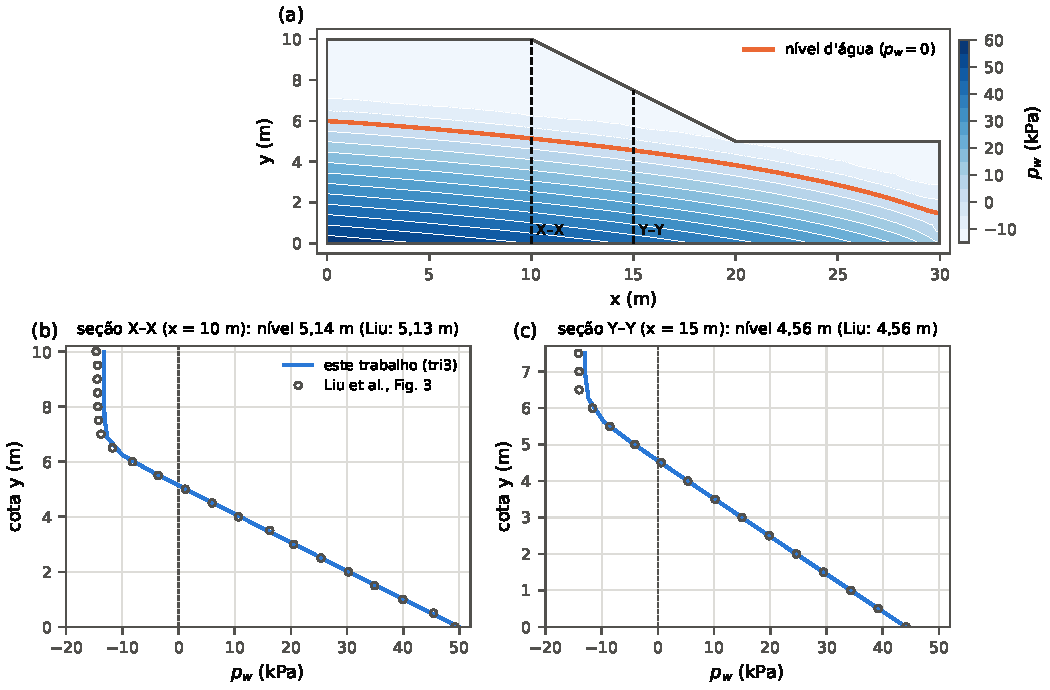
\includegraphics[width=\linewidth]{figs/fig_pressoes.pdf}
\caption{O permanente das médias (tri3). (a) $p_w$ e o nível d'água ($p_w = 0$) no talude, com as seções da Fig.~1 de
Liu. (b, c) $p_w$ nas seções X--X e Y--Y, contra a Fig.~3 de Liu (``This study'', lida dos pixels da figura raster;
erro de leitura de $\approx 0{,}3$~kPa).}
\label{fig:pressoes}
\end{figure}

\clearpage
\section{A probabilidade de falha por método}\label{sec:prob}
% gerado por gera_dados.py; nao edite
\begin{table}[htbp]\centering\footnotesize\setlength{\tabcolsep}{4pt}
\caption{$P_f = P(FS < 1)$ do caso B ($\alpha = 0^\circ$, $q/k_s = 0{,}01$) por método, contra as Tabelas 2 e 4 de Liu. LS: IC de 95\,\% na escala log ($P_f\, e^{\pm 1{,}96 s}$, $s^2 = \ln(1 + CoV^2)$; o normal tem limite inferior negativo com $CoV > 51\,\%$). MC: IC de Wilson. Ajustes: a Eq.~13 de Liu (lognormal) e a normal com a média e o desvio do nosso MC. A Tabela 2 é a verificação no modelo do cenário 3.}\label{tab:pf}
\begin{tabular}{llll}\toprule
método & detalhe & cenário 2 ($c'$, $\varphi'$) & cenário 3 ($c'$, $\varphi'$, $k_s$) \\\midrule
FORM modal & $\beta$; $\Phi(-\beta)$ & 4{,}82; \ensuremath{7{,}1\times 10^{-7}} & 4{,}77; \ensuremath{9{,}3\times 10^{-7}} \\
line sampling & 600 e 600 linhas & \ensuremath{9{,}3\times 10^{-6}} ($CoV$ 54\,\%) & \ensuremath{2{,}6\times 10^{-5}} ($CoV$ 34\,\%) \\
 & IC 95\,\% (log) & [\ensuremath{3{,}5\times 10^{-6}}; \ensuremath{2{,}5\times 10^{-5}}] & [\ensuremath{1{,}4\times 10^{-5}}; \ensuremath{5{,}0\times 10^{-5}}] \\
 & $-\Phi^{-1}(P_f)$ & 4{,}28 & 4{,}04 \\
MC direto & falhas & 0 em 2\,500 & 0 em 10\,000 \\
 & IC 95\,\% (Wilson) & [0; \ensuremath{1{,}5\times 10^{-3}}] & [0; \ensuremath{3{,}8\times 10^{-4}}] \\
 & média $\pm$ desvio do FS & 1{,}550 $\pm$ 0{,}155 & 1{,}538 $\pm$ 0{,}159 \\
ajuste ao nosso MC & lognormal: $\beta$; $P_f$ & 4{,}35; \ensuremath{6{,}9\times 10^{-6}} & 4{,}11; \ensuremath{2{,}0\times 10^{-5}} \\
 & normal: $P_f$ & \ensuremath{1{,}9\times 10^{-4}} & \ensuremath{3{,}7\times 10^{-4}} \\
\midrule Liu, Tabela 4 & lognormal (2000): $\beta$; $P_f$ & 3{,}95; \ensuremath{4{,}08\times 10^{-5}} & 3{,}68; \ensuremath{1{,}19\times 10^{-4}} \\
Liu, Tabela 2 & LHS, 2\,500 amostras & -- & \ensuremath{4{,}0\times 10^{-3}} \\
 & CDF ajustada & -- & \ensuremath{4{,}58\times 10^{-3}} \\
\bottomrule\end{tabular}\end{table}

\begin{itemize}
  \item \textbf{FORM modal:} $\beta = \betaDois$ no cenário 2 e \betaTres{} no 3, com $\Phi(-\beta)$ de \pfFORMDois{} e
    \pfFORMTres. A importância fica em $\varphi'$ ($\alpha^2_{\varphi} = \alfaPhiDois$; $\alpha^2_c = \alfaCDois$). O
    termo de $k_s$ sai nulo, porque o gradiente modal congela as pressões. O $\Phi(-\beta)$ fica \razaoFORMDois{} e \razaoFORMTres{} vezes abaixo do LS:
    o estado limite não é plano, e as raízes das linhas se espalham em torno do $\beta$ (Fig.~\ref{fig:raizes}a).
  \item \textbf{Line sampling (Figs.~\ref{fig:conv} e \ref{fig:raizes}):} \pfLSDois{} ($CoV = \cvLSDois\,\%$) no
    cenário 2 e \pfLSTres{} ($CoV = \cvLSTres\,\%$) no 3, com \linhasDois{} linhas cada. As raízes das linhas vão de
    \cMinDois{} a \cMaxDois{} (cenário 2), com mediana \cMedDois, perto do $\beta$ do FORM. As poucas linhas com raiz
    abaixo de 4 dão quase toda a $P_f$: no cenário 2, \nCquatroDois{} linhas dão \fracCquatroDois\,\% dela, e uma
    sozinha responde por \fracMaiorDois\,\%; no 3, \nCquatroTres{} linhas dão \fracCquatroTres\,\%. Daí o $CoV$ alto. A nova campanha estende os dois cenários a $\approx 2000$ linhas;
    este relatório se refaz com as linhas que existirem (\texttt{gera.sh}).
  \item \textbf{MC direto:} nenhuma falha. O menor FS das realizações é \minMCDois{} (cenário 2) e \minMCTres{} (3). O
    limite superior de Wilson é \wilsonDois{} e \wilsonTres{}, coerente com o LS.
  \item \textbf{Contra Liu:} as nossas $P_f$ ficam \razaoTabQuatroDois{} e \razaoTabQuatroTres{} vezes abaixo da
    Tabela~4, e, no cenário 3, duas ordens de grandeza abaixo da verificação da Tabela~2 (Fig.~\ref{fig:pf}). As
    Seções~\ref{sec:mc} e~\ref{sec:porque} tratam das duas diferenças.
\end{itemize}

\begin{figure}[htbp]\centering
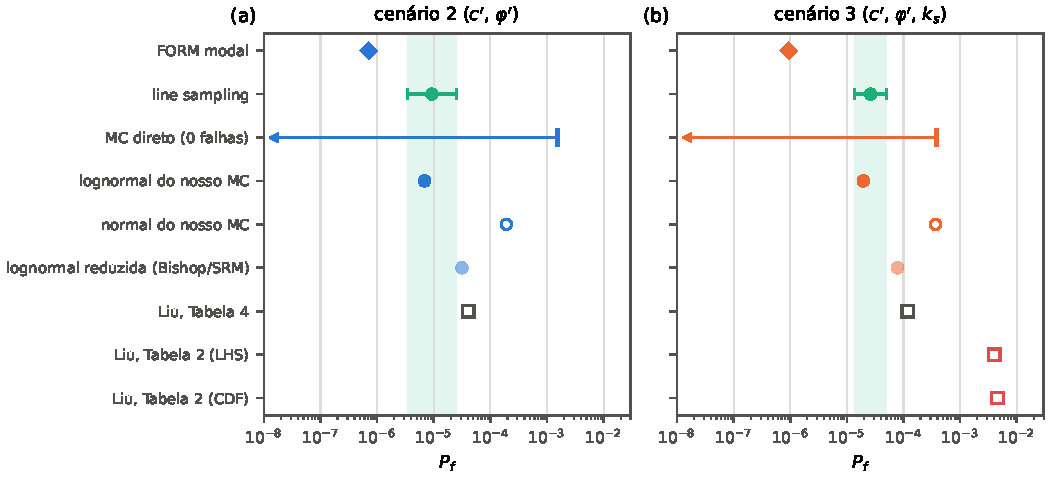
\includegraphics[width=\linewidth]{figs/fig_pf.pdf}
\caption{$P_f$ por método, em escala log. LS: IC de 95\,\% na escala log (faixa verde). MC: nenhuma falha; a seta vai
até o limite superior de Wilson. Lognormal reduzida: o nosso FS vezes $1{,}525/\fsDet$, com o mesmo $CoV$. Quadrados:
Liu (Tabela~4; Tabela~2, só no modelo do cenário 3).}
\label{fig:pf}
\end{figure}

\begin{figure}[htbp]\centering
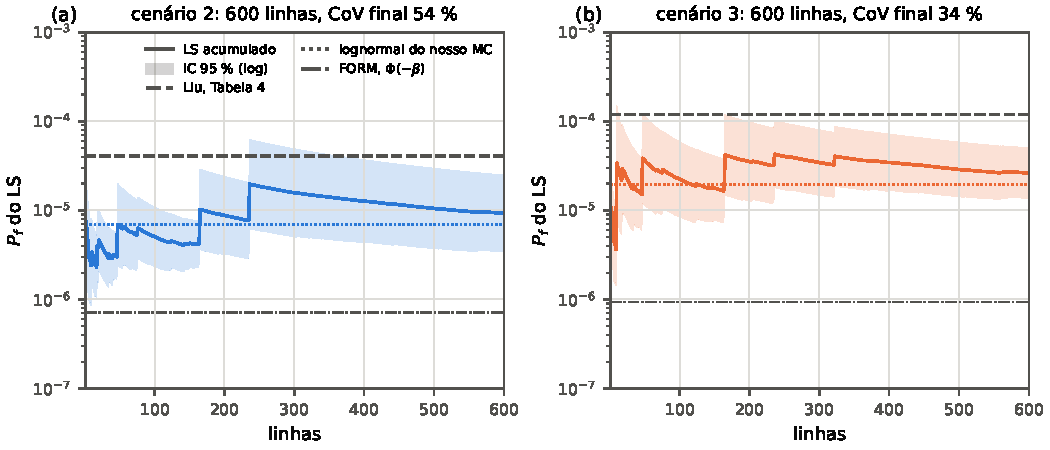
\includegraphics[width=\linewidth]{figs/fig_convergencia.pdf}
\caption{Convergência do LS: a $P_f$ acumulada contra o número de linhas, com o IC de 95\,\% na escala log. Os saltos
são as linhas de raiz pequena.}
\label{fig:conv}
\end{figure}

\begin{figure}[htbp]\centering
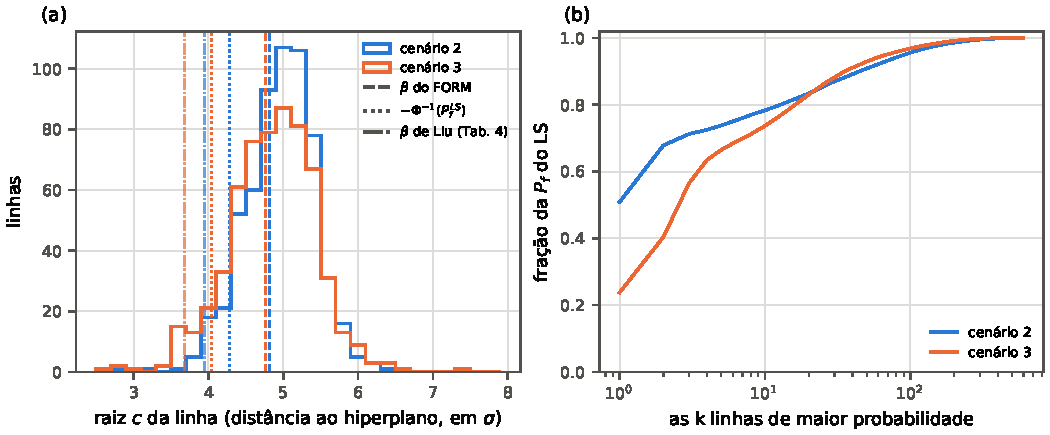
\includegraphics[width=\linewidth]{figs/fig_raizes.pdf}
\caption{(a) As raízes $c$ das linhas do LS, contra o $\beta$ do FORM, o índice equivalente do LS e o $\beta$ da
Tabela~4 de Liu. (b) A fração da $P_f$ do LS que vem das $k$ linhas de maior probabilidade.}
\label{fig:raizes}
\end{figure}

\clearpage
\section{O que o MC direto prova: a Tabela 2 de Liu fica excluída}\label{sec:mc}
\begin{itemize}
  \item \textbf{A verificação de Liu:} a Tabela~2 dá $P_f = 4{,}0 \times 10^{-3}$ por hipercubo latino com 2500
    amostras (a mesma de Jiang et al.~\cite{jiang2014}) e \pfTabDoisCDF{} pela CDF ajustada, para o modelo do cenário
    3, que o artigo diz ser ``the same'' de Jiang. A Tabela~4 dá $1{,}19 \times 10^{-4}$ para o mesmo cenário,
    \razaoTabDois{} vezes menos. As duas não fecham.
  \item \textbf{O nosso MC do cenário 3:} \nMCTres{} realizações, nenhuma falha. Se a $P_f$ fosse $4{,}0 \times
    10^{-3}$, esperaríamos \nTabDoisTres{} falhas, e a chance de nenhuma seria $(1 - 0{,}004)^{10\,000} =
    \pZeroTabDoisTres$. Com a $P_f$ da Tabela~4, a chance de nenhuma falha é \pZeroTabQuatroTres: o MC é compatível com
    a Tabela~4 e exclui a Tabela~2. O limite de Wilson, \wilsonTres, fica 10 vezes abaixo de $4 \times 10^{-3}$.
  \item \textbf{O próprio artigo concorda:} na Fig.~11 de Liu, o menor FS das 2000 realizações do cenário 3 é
    $\approx \liuMinTres$, ou seja, nenhuma falha em 2000. Com $P_f = 4 \times 10^{-3}$, a chance disso seria
    \pZeroLiu.
  \item \textbf{A diferença de modelo não salva a Tabela~2:} o nosso FS fica \difDet\,\% acima do de Liu, o que baixa a
    nossa $P_f$. Mas, mesmo reduzido pela razão Bishop/SRM, ele dá \pfLNredTres{} (lognormal),
    \razaoTabDoisRedTres{} vezes abaixo de $4 \times 10^{-3}$. Nem a normal com a média e o desvio do próprio Liu chega lá (\liuPfNTres). Os $4 \times
    10^{-3}$ só cabem num modelo diferente, como o de Jiang, se ele não for de fato o mesmo (outras escalas, outro núcleo
    ou outro $\varphi^b$; o artigo de Jiang é em chinês e não foi lido).
\end{itemize}

\section{Por que ficamos abaixo da Tabela 4}\label{sec:porque}
\begin{itemize}
  \item \textbf{O desvio é o mesmo (Tabela~\ref{tab:aprox} e Fig.~\ref{fig:hist}):} o nosso FS tem desvio \sdDois{}
    (cenário 2) e \sdTres{} (3); a Fig.~11 de Liu dá \liuSdDois{} e \liuSdTres. Os $CoV$ ficam em 10 a 10,5\,\% nos dois
    lados. Ao contrário do caso A, o espalhamento do FS concorda.
  \item \textbf{A média não:} a Fig.~11 não mostra a média, mas a Eq.~13 de Liu, com o desvio da figura e o $\beta$ da
    Tabela~4, exige médias de \liuMuDois{} e \liuMuTres. As nossas são \muDois{} e \muTres{}, \redLiuMu\,\% acima no
    cenário 2. É a mesma diferença do determinístico (\difDetRel\,\%; o Bishop das médias dá 1,525 e o nosso SRM
    \fsDetTres). A média do FS fica abaixo do FS das médias nos dois lados: \muDois{} contra \fsDetTres{} aqui, \liuMuDois{} contra
    1,525 em Liu.
  \item \textbf{O peso da média no $\beta$:} com $CoV = 0{,}10$, $d\beta/d\ln\mu = 1/\zeta \approx \dbetaDois$
    ($\zeta^2 = \ln(1 + CoV^2)$). Uma média \difDetRel\,\% menor baixa o $\beta$ em $\approx 0{,}34$ e multiplica a
    $P_f$ por 4 a 5. Com o nosso FS reduzido pela razão Bishop/SRM e o mesmo $CoV$, a lognormal dá $\beta =
    \betaLNredDois$ e $P_f = \pfLNredDois$ no cenário 2 (Tabela~4: 3,95 e $4{,}08 \times 10^{-5}$). No cenário 3, dá
    \betaLNredTres{} e \pfLNredTres{} (Tabela~4: 3,68 e $1{,}19 \times 10^{-4}$). O que sobra são os fatores de
    \razaoTabQuatroRedDois{} e \razaoTabQuatroRedTres, dentro da diferença entre as médias implícitas
    (\redReqDois{} e \redReqTres\,\% seriam necessários) e da leitura da Fig.~11.
  \item \textbf{A lognormal contra o nosso LS:} ajustada ao nosso MC pela Eq.~13, ela dá \pfLNDois{} (cenário 2) e
    \pfLNTres{} (3), \razaoLNLSDois{} da $P_f$ do LS nos dois casos, dentro do IC do LS. A assimetria do nosso FS
    (\assimDois{} e \assimTres) é a da lognormal com esse $CoV$ (\assimLN). Neste problema, então, o ajuste lognormal
    de Liu é uma boa aproximação da cauda, e o método de confiabilidade não explica a diferença. A normal, por outro
    lado, erra para cima \razaoNLSTres{} a \razaoNLSDois{} vezes (\pfNDois{} e \pfNTres).
  \item \textbf{Em resumo:} a diferença para a Tabela~4 é a diferença de \difDetRel\,\% no FS das médias (SRM contra
    Bishop), amplificada pela cauda. Ela não está no espalhamento do FS, nem na forma da distribuição, nem no método.
\end{itemize}

% gerado por gera_dados.py; nao edite
\begin{table}[htbp]\centering\footnotesize\setlength{\tabcolsep}{4pt}
\caption{As aproximações lognormal (Eq.~13 de Liu) e normal a partir da média e do desvio do FS. ``Reduzido'': o nosso FS multiplicado por $1{,}525/1{,}5785$ (Bishop/SRM no determinístico), com o mesmo $CoV$. Liu: o desvio da Fig.~11 e a média que a Eq.~13 exige para o $\beta$ da Tabela 4. Última coluna: a $P_f$ de referência de cada linha (o nosso LS; a Tabela 4).}\label{tab:aprox}
\begin{tabular}{llrrrrrrr}\toprule
cenário & FS & média & desvio & $CoV$ (\%) & $\beta_{LN}$ & $P_f$ lognormal & $P_f$ normal & referência \\\midrule
cenário 2 & nosso MC & 1{,}550 & 0{,}155 & 10{,}0 & 4{,}35 & \ensuremath{6{,}9\times 10^{-6}} & \ensuremath{1{,}9\times 10^{-4}} & LS \ensuremath{9{,}3\times 10^{-6}} \\
 & reduzido & 1{,}497 & 0{,}149 & 10{,}0 & 4{,}00 & \ensuremath{3{,}1\times 10^{-5}} & \ensuremath{4{,}4\times 10^{-4}} & \\
 & Liu & 1{,}489 & 0{,}148 & 10{,}0 & 3{,}95 & \ensuremath{3{,}9\times 10^{-5}} & \ensuremath{5{,}0\times 10^{-4}} & Tab.~4: \ensuremath{4{,}08\times 10^{-5}} \\
\midrule
cenário 3 & nosso MC & 1{,}538 & 0{,}159 & 10{,}4 & 4{,}11 & \ensuremath{2{,}0\times 10^{-5}} & \ensuremath{3{,}7\times 10^{-4}} & LS \ensuremath{2{,}6\times 10^{-5}} \\
 & reduzido & 1{,}486 & 0{,}154 & 10{,}4 & 3{,}78 & \ensuremath{7{,}8\times 10^{-5}} & \ensuremath{8{,}0\times 10^{-4}} & \\
 & Liu & 1{,}478 & 0{,}155 & 10{,}5 & 3{,}68 & \ensuremath{1{,}2\times 10^{-4}} & \ensuremath{1{,}0\times 10^{-3}} & Tab.~4: \ensuremath{1{,}19\times 10^{-4}} \\
\bottomrule\end{tabular}\end{table}


\begin{figure}[htbp]\centering
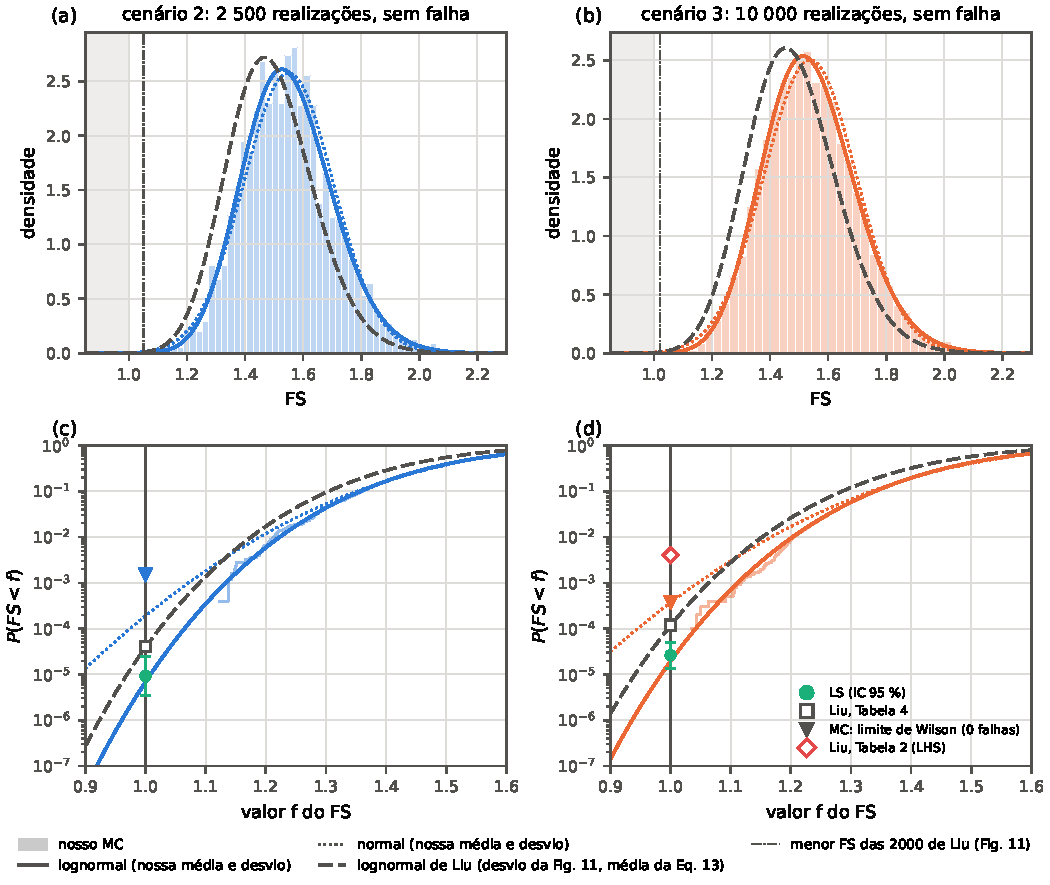
\includegraphics[width=\linewidth]{figs/fig_hist.pdf}
\caption{O FS do MC direto. (a, b) Histograma, contra a lognormal e a normal com a nossa média e desvio e contra a
lognormal implícita de Liu (o desvio da Fig.~11 e a média que a Eq.~13 exige para o $\beta$ da Tabela~4). A faixa cinza
é a falha; a linha traço-ponto, o menor FS das 2000 realizações de Liu. (c, d) A cauda, $P(FS < f)$: a escada é o nosso
MC; em $f = 1$, o LS, o limite de Wilson do MC e as $P_f$ de Liu.}
\label{fig:hist}
\end{figure}

\clearpage
\section{O efeito do campo de $k_s$}\label{sec:k}
\begin{itemize}
  \item \textbf{Na $P_f$:} o campo de $k_s$ multiplica a $P_f$ do LS por \razaoLS{} (do cenário 2 ao 3; o $CoV$ da razão
    é de \razaoLScv\,\%). Liu tem \razaoTabQuatro{} (Tabela~4). O efeito relativo concorda, mesmo com as $P_f$ abaixo.
  \item \textbf{No FS, realização a realização (Fig.~\ref{fig:k}a):} nas \nPar{} realizações pareadas (os mesmos $c'$ e
    $\varphi'$), a correlação entre os FS dos dois cenários é \parCorr. O campo de $k_s$ muda o FS em \parDmu{} na média,
    com desvio de \parDsd{} (95\,\% entre \parDlo{} e \parDhi). O desvio do FS sobe de \parSdDois{} a \parSdTres. É
    esse pequeno alargamento, somado à média um pouco menor, que pesa na cauda.
  \item \textbf{No nível d'água (Fig.~\ref{fig:k}b):} com $k_s$ fixo, o nível fica em 5,1~m na crista e 4,5~m na meia
    altura (a saída do MC tem resolução de 0,1~m). Com o campo, ele varia: $\nivXXmuTres \pm \nivXXsdTres$~m na crista
    (95\,\% entre \nivXXloTres{} e \nivXXhiTres~m) e $\nivYYmuTres \pm \nivYYsdTres$~m na meia altura (entre
    \nivYYloTres{} e \nivYYhiTres~m). Um $k_s$ menor perto da face sobe o nível e baixa o FS.
  \item \textbf{No FORM:} o gradiente modal tem termo nulo em $k_s$ (as pressões ficam congeladas), então a direção do
    FORM é a mesma nos dois cenários. O $\beta$ cai de \betaDois{} a \betaTres{} só porque o centro ($\xi = 0$) usa a
    mediana de $k_s$, abaixo da média. O LS continua sem viés: as linhas amostram todos os modos, inclusive os de $k_s$,
    no hiperplano. O efeito do $k_s$ aparece nas raízes: no cenário 3, 5\,\% das linhas ficam abaixo de
    \cPcincoTres{}, contra \cPcincoDois{} no 2 (Fig.~\ref{fig:raizes}a).
  \item \textbf{O custo:} o cenário 3 resolve um permanente por análise, mas o tempo mediano por análise (\tempoTres~s)
    é o mesmo do cenário 2 (\tempoDois~s): o SRM domina.
\end{itemize}

\begin{figure}[htbp]\centering
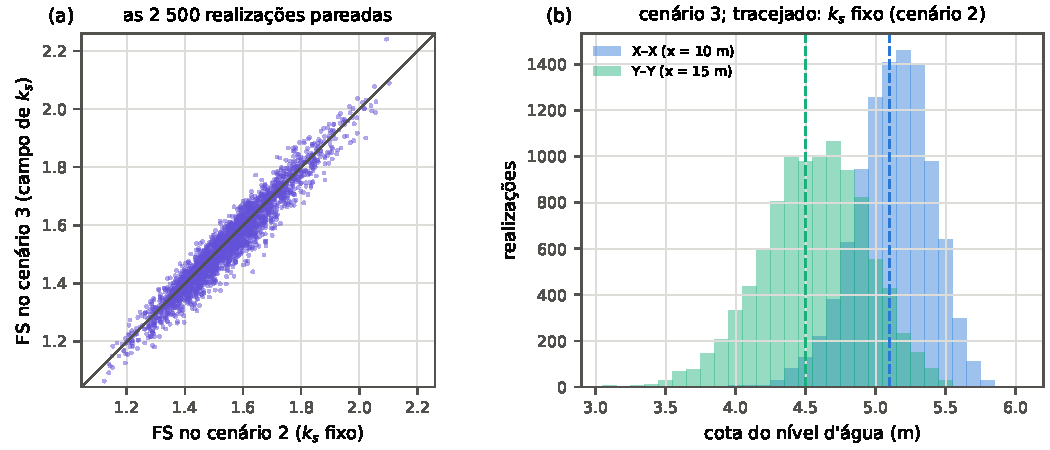
\includegraphics[width=\linewidth]{figs/fig_k.pdf}
\caption{O efeito do campo de $k_s$. (a) O FS das realizações pareadas do MC (os mesmos $c'$ e $\varphi'$): cenário 3
contra cenário 2. (b) O nível d'água nas seções X--X e Y--Y no cenário 3; tracejado: o nível com $k_s$ fixo.}
\label{fig:k}
\end{figure}

\section{Conclusões e próximos passos}\label{sec:conclusoes}
\begin{itemize}
  \item \textbf{Determinístico:} o permanente reproduz a Fig.~3 de Liu (o nível d'água a 0,01~m nas duas seções). O FS
    das médias fica \difDet\,\% acima do Bishop (\fsDet{} contra 1,525).
  \item \textbf{$P_f$:} LS com \pfLSDois{} e \pfLSTres{} nos cenários 2 e 3, coerente com o MC direto sem falhas
    (limites de Wilson de \wilsonDois{} e \wilsonTres) e com a lognormal ajustada ao nosso MC.
  \item \textbf{A Tabela~2 de Liu ($4 \times 10^{-3}$) está errada para o modelo publicado:} o MC de \nMCTres{}
    realizações a exclui, e a Fig.~11 do próprio artigo também. A referência de $P_f$ do caso B é a Tabela~4.
  \item \textbf{A Tabela~4 se explica:} o $CoV$ do FS é o mesmo, e a diferença de \difDetRel\,\% na média (SRM contra
    Bishop) dá o fator 4 a 5 na $P_f$. Com o FS reduzido por essa razão, a lognormal fica a \razaoTabQuatroRedDois{} e
    \razaoTabQuatroRedTres{} da Tabela~4. O efeito do campo de $k_s$ (\razaoLS{} contra \razaoTabQuatro) concorda.
  \item \textbf{O LS precisa de mais linhas:} 600 linhas dão $CoV$ de \cvLSDois{} e \cvLSTres\,\%, porque poucas linhas
    de raiz pequena carregam a $P_f$. A extensão para $\approx 2000$ linhas já está prevista no fermi; com ela, rodar o
    \texttt{baixar\_liu2024.sh} e o \texttt{gera.sh}.
  \item \textbf{Próximos passos:}
    \begin{itemize}
      \item um FS por equilíbrio limite (Bishop) no mesmo permanente, para medir a diferença de 3,4\,\% sem a busca do
        SLOPE/W, e conferir se o mecanismo crítico é o de base;
      \item ler o modelo de Jiang et al.~\cite{jiang2014} para saber de onde vêm os $4 \times 10^{-3}$;
      \item os ângulos $\alpha = 30^\circ$ e $150^\circ$ da Tabela~4 (o núcleo girado já está no
        \texttt{nystrom\_base.py}), se o caso B for usado além da verificação.
    \end{itemize}
\end{itemize}

\begin{thebibliography}{9}
\bibitem{liu2024} L.-L.~Liu, H.~Han, S.-Y.~Huang, L.~Huang, Y.-M.~Cheng. Combined influence of rotated transverse
  anisotropy in mechanical parameters and hydraulic conductivity of soils on reliability evaluation of an unsaturated
  slope under rainfalls. \emph{Computers and Geotechnics}, 165:105938, 2024. doi:10.1016/j.compgeo.2023.105938.
\bibitem{jiang2014} S.-H.~Jiang, D.-Q.~Li, C.-B.~Zhou, L.-M.~Zhang. Reliability analysis of unsaturated slope
  considering spatial variability (em chinês). \emph{Rock and Soil Mechanics}, 35(9):2569--2578, 2014.
\bibitem{cho2010} S.~E.~Cho. Probabilistic assessment of slope stability that considers the spatial variability of
  soil properties. \emph{Journal of Geotechnical and Geoenvironmental Engineering}, 136(7):975--984, 2010.
\bibitem{hasofer1974} A.~M.~Hasofer, N.~C.~Lind. Exact and invariant second-moment code format. \emph{Journal of the
  Engineering Mechanics Division (ASCE)}, 100(1):111--121, 1974.
\bibitem{rackwitz1978} R.~Rackwitz, B.~Fiessler. Structural reliability under combined random load sequences.
  \emph{Computers \& Structures}, 9(5):489--494, 1978.
\bibitem{koutsourelakis2004} P.~S.~Koutsourelakis, H.~J.~Pradlwarter, G.~I.~Schuëller. Reliability of structures in
  high dimensions, part~I: algorithms and applications. \emph{Probabilistic Engineering Mechanics}, 19(4):409--417,
  2004. doi:10.1016/j.probengmech.2004.05.001.
\bibitem{wilson1927} E.~B.~Wilson. Probable inference, the law of succession, and statistical inference.
  \emph{Journal of the American Statistical Association}, 22(158):209--212, 1927.
\bibitem{formulacao} Campos aleatórios e confiabilidade de taludes: as bases de Karhunen--Loève (analítica e Nyström),
  o FORM com gradiente modal (SRM e GIM) e o line sampling. Documento interno,
  \path{docs/confiabilidade_campos/formulacao/formulacao.pdf}, 2026.
\bibitem{exemplos} Exemplos probabilísticos de chuva não saturada (a especificação dos casos A, B e C). Relatório
  interno, \path{~/Dropbox/UnsaturatedSoil/referencias/referencias_selecionadas_claude/reports/}, 2026.
\end{thebibliography}

\appendix
\section{Arquivos e como refazer}
\begin{itemize}
  \item \textbf{A especificação} do caso B é a seção ``B)'' do relatório dos exemplos~\cite{exemplos}. As Figs.~3 e 11
    de Liu, lidas dos pixels das figuras raster do PDF, estão em \path{liu2024/dados} (\texttt{liu\_fig3\_pwp.csv} e
    \texttt{liu\_fig11.csv}, com o método de leitura no cabeçalho).
  \item \textbf{A campanha:} \path{Projects/SlopeRandomFieldRefinement/cluster/liu2024_casos.sbatch}, com os cenários
    em \path{casos_liu2024.txt}; saída no fermi em \path{$DATA/liu2024}, baixada (\texttt{baixar\_liu2024.sh}) em
    \path{~/projects/runs/fermi_liu2024}.
  \item \textbf{As conferências no PC:} \path{~/projects/runs/liu2024} (\path{det/}: as malhas, a chuva vertical, o
    $\psi_{aev}$, $\varphi^b = 0$ e o perfil de $p_w$, \texttt{perfil.py}; \path{piloto/}: 3 contra 4 níveis no fator,
    0,05 a 0,3\,\% no FS; \path{nystrom/}; \path{form/}).
  \item \textbf{Este relatório:} \texttt{gera.sh} refaz o resumo (\texttt{resumo\_liu2024.py}) sobre a campanha baixada,
    roda o \texttt{gera\_dados.py} (tabelas em \path{tab/}, números em \path{numeros.tex}, figuras em \path{figs/}) e
    o \LaTeX. O LS entra com as linhas que existirem no \texttt{linhas.csv}.
\end{itemize}
\end{document}
